\section{Essential position control}

This experiment covers angle reference following for a single link in contact with an obstacle. The motivation is to show the impact of the mapping to the essential position space within the allowable position space. In other words, the use of the filter $\prescript{}{j}{\mathbf{F}}_{p}$ from (\ref{eq:hpfc_fp}). This method is also described in more detail in \ref{subsec:task-oriented}.

Link number 5, which is in contact with the foremost obstacle, is controlled to a constant angle $\theta_{t,d,3}$ measured with respect to the base frame. The controlled variable is referred to as $\theta_{t,3}$, and is the only essential variable the mentioned filter takes into account in this example. A simulation without the filter is also included to show the importance of defining which variables are essential for a given task when the total number of variables that \textit{could} be controlled are greater than the number of actuated joints.

The setup for this experiment is presented in Table \ref{tab:exp_single_pos}. It should b noted that the force control is left out for this experiment.

\begin{table}[]
    \centering
    \begin{tabular}{|c|c|c|}
        \hline
        & Value & Unit\\
        \hline
        Number of obstacles & $3$ & \\
        Number of links & $6$ & \\
        Initial joint angles & $\mathbf{0}_{13 \times 1}$ & $[rad]$ \\
        $\theta_{t,3,d}$ & $0.3$ & $[rad]$ \\
        $[K_p, K_i]$ & $[0.05, 0.005]$ &\\
        Essential variables & $[\theta_{t,3}]$ & $[rad]$ \\
        \hline
    \end{tabular}
    \caption{Simulation configuration for position control experiment}
    \label{tab:exp_single_pos}
\end{table}

The global contact link angle, joint angles and joint torques for the experiments are shown in Figures \ref{fig:singlepos} and \ref{fig:singlepos-nofilter}. As one could imagine, the latter shows the unfiltered control case. The contact link is quite far from reaching its reference and the control does not seem to be very meaningful for the purpose. The corresponding joint angle values show that the snake simply turns its first actuated joint, resulting in the tail of the snake robot spinning around before getting stuck. The behavior of the snake robot in the filtered example makes more sense, as it simply bends the joint preceding to the link and compensates by bending the following joint in the opposite direction.

The configuration of the snake robot at the end of the filtered and unfiltered simulations is better visualized in Figures \ref{fig:singlepos-gazebo} and \ref{fig:singlepos-gazebo-nofilter} respectively. From the last figure it is also evident that the robot has lost contact with some of the obstacles, which means that the mathematical model the controller is based on no longer is valid.

\begin{figure}
    \centering
    
    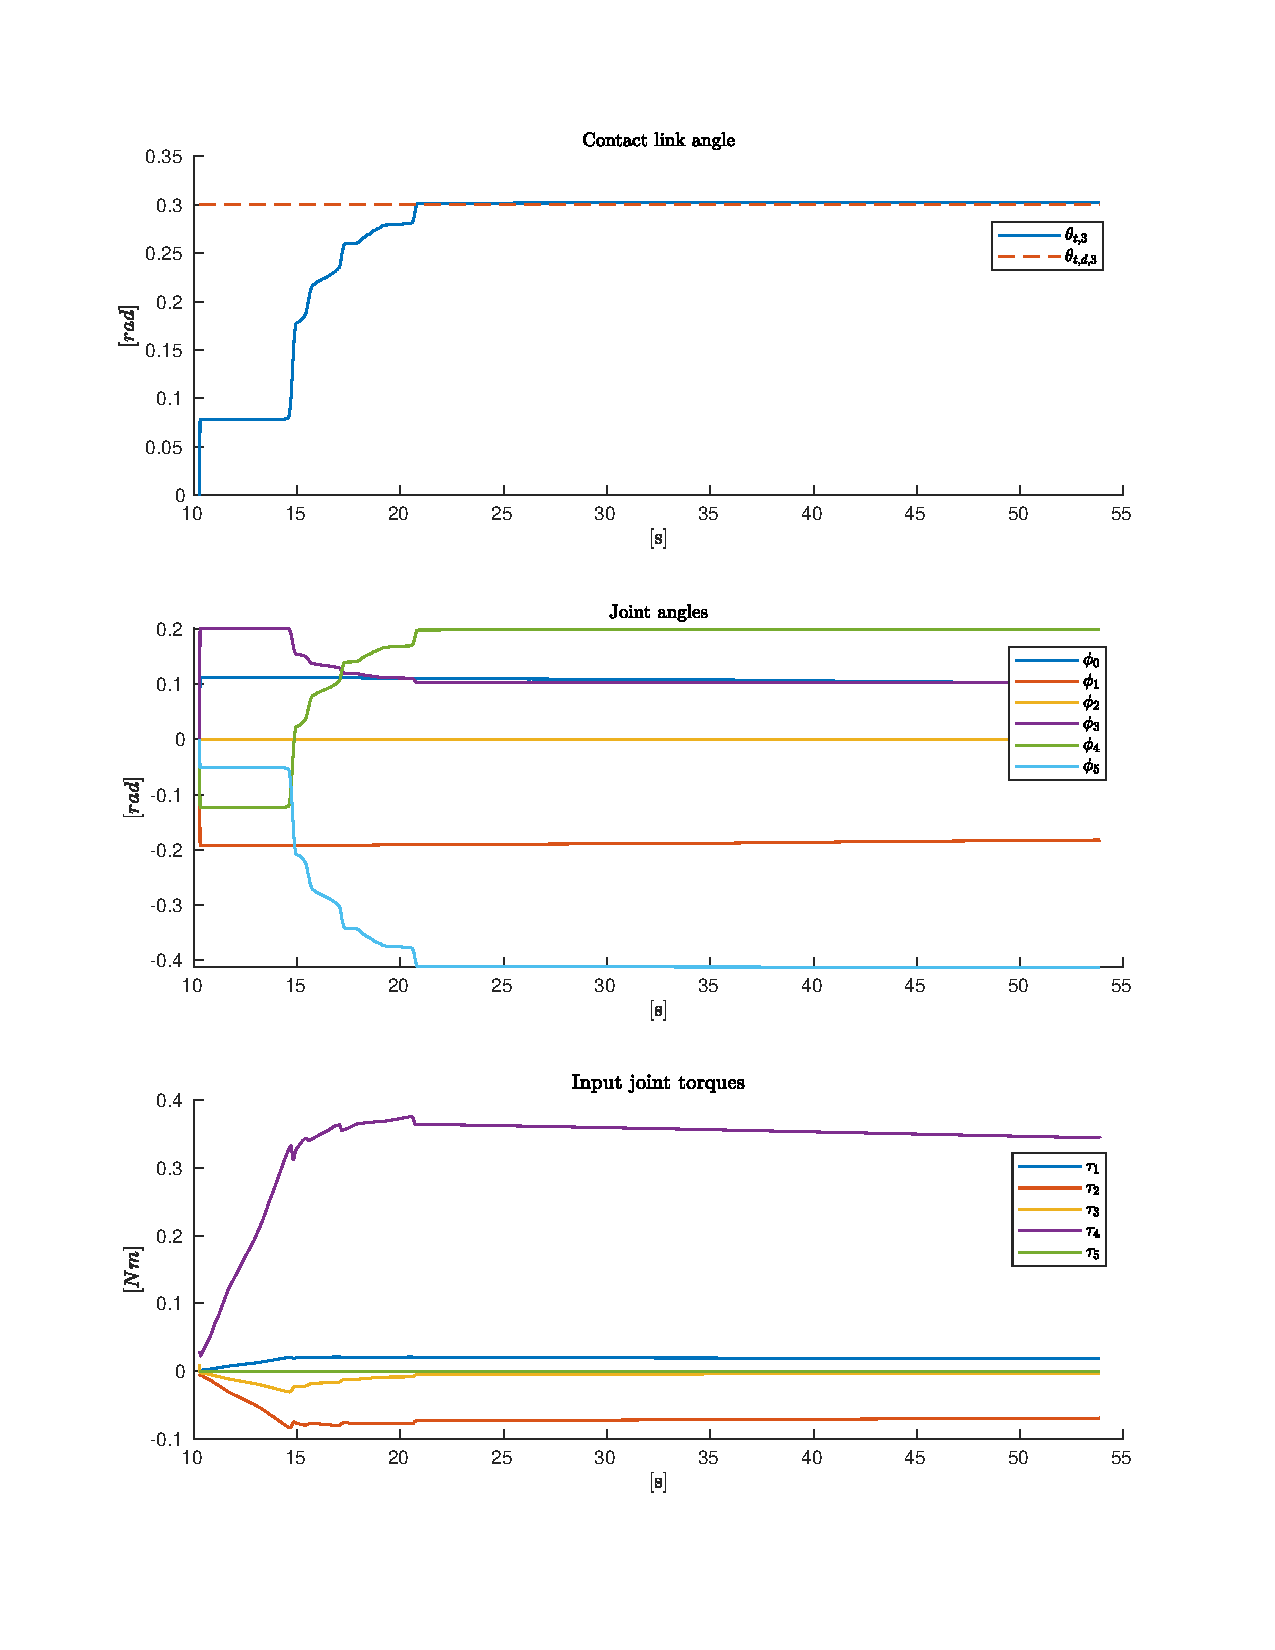
\includegraphics[trim=2cm 2cm 2cm 2cm, clip=true, width=\textwidth]{figures/experiments/single_pos/single-pos-3plot.pdf}

    \caption{Filtered position control}
    \label{fig:singlepos}
\end{figure}

\begin{figure}
    \centering
    
    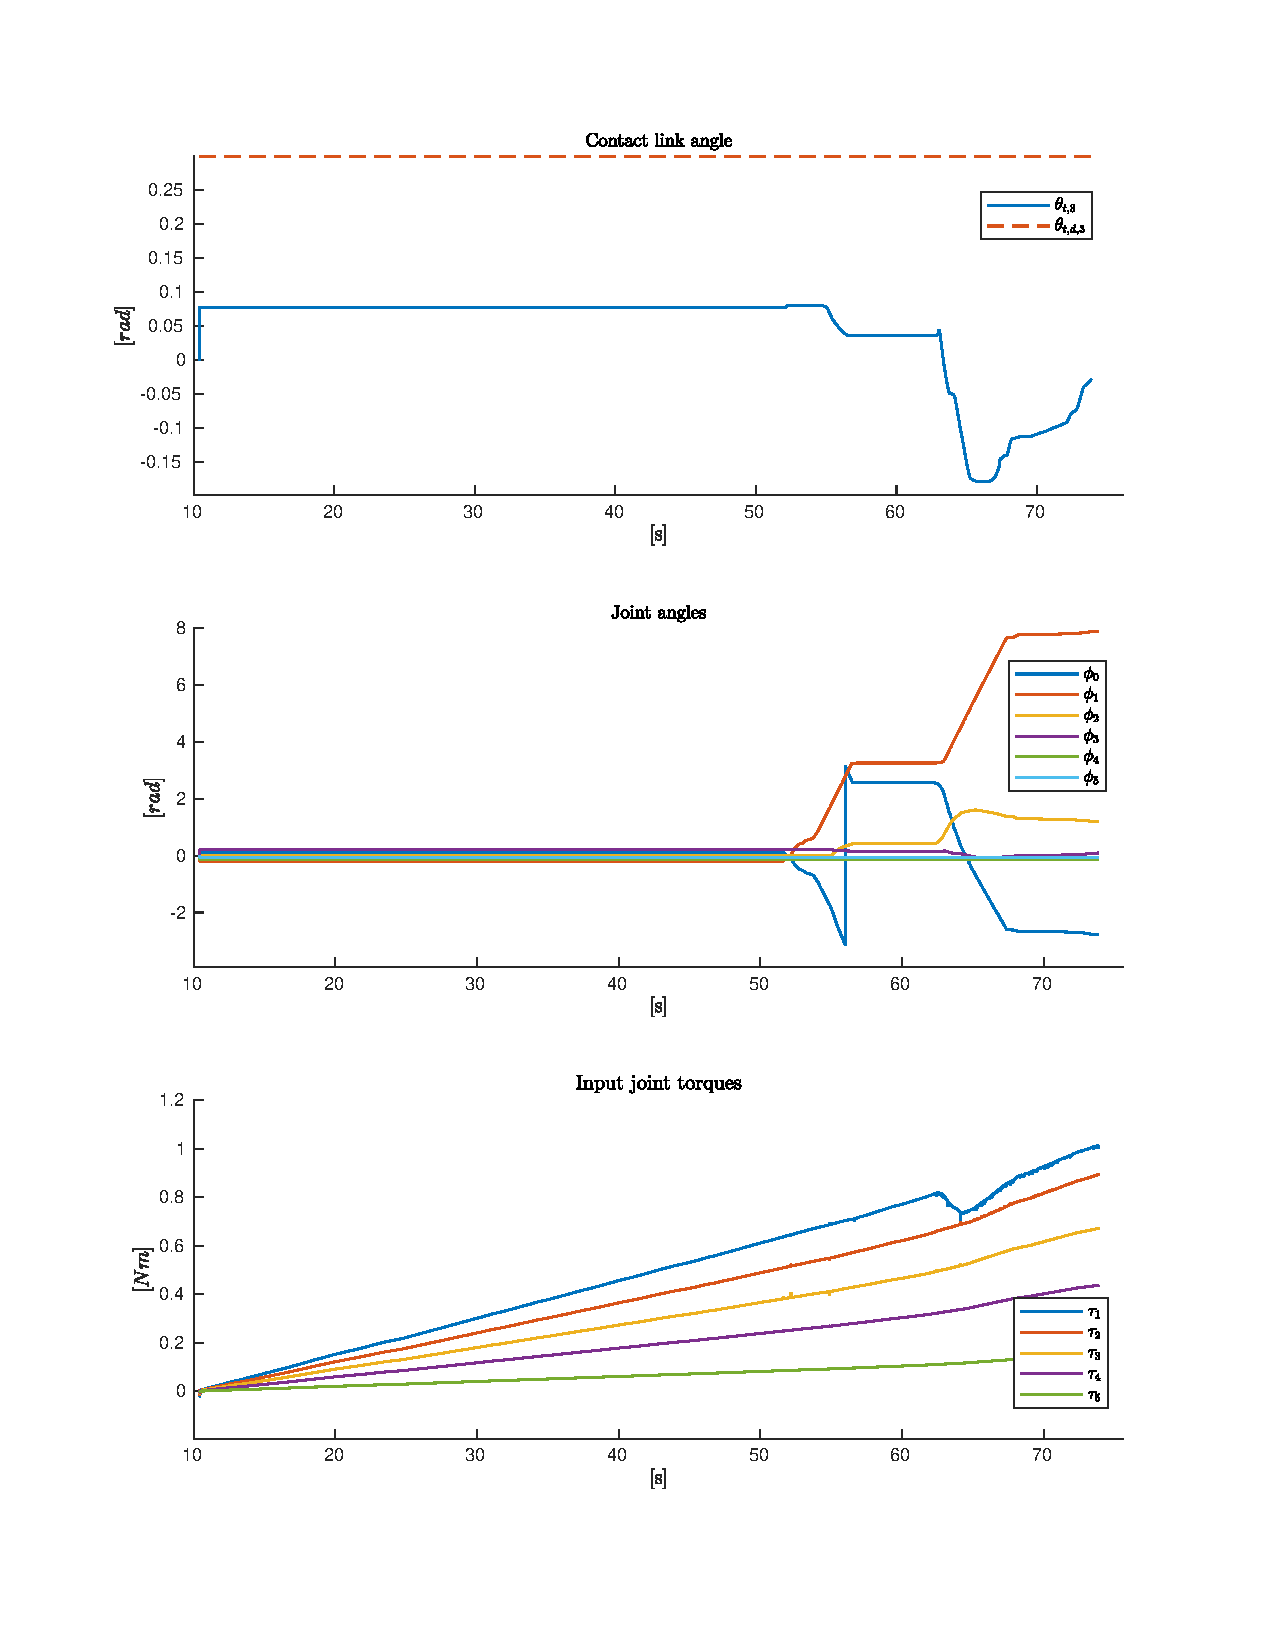
\includegraphics[trim=2cm 2cm 2cm 2cm, clip=true, width=\textwidth]{figures/experiments/single_pos/single-pos-3plot-fail.pdf}

    \caption{Unfiltered position control}
    \label{fig:singlepos-nofilter}
\end{figure}

\begin{figure}
    \centering
    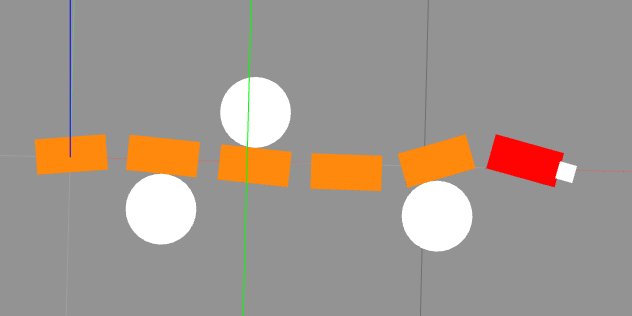
\includegraphics[width=0.5\textwidth]{figures/experiments/single_pos/gazebo_single_pos.png}
    \caption{Snake robot after filtered position control}
    \label{fig:singlepos-gazebo}
\end{figure}

\begin{figure}
    \centering
    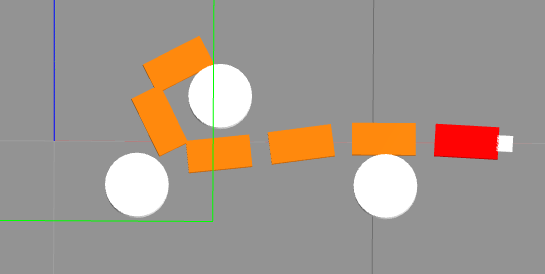
\includegraphics[width=0.5\textwidth]{figures/experiments/single_pos/gazebo_single_pos_nofilter.png}
    \caption{Snake robot after unfiltered position control}
    \label{fig:singlepos-gazebo-nofilter}
\end{figure}

The explanation for these results is that the unfiltered case tries to control all possible position variables in $\mathbf{r}$, meaning all contact link angles and the translational position along every contact point. This sums up to 6 variables. However, the robot only has 5 actuators. Furthermore, the last actuator can not be taken into account since it is after the last contact point. This results in a total of 4 actuators that can be utilized for the control. 
Needless to say, trying to control 6 variables is infeasible for this snake robot. Increasing the number of joints and links would give it a much better basis for achieving this task.

%In this snake robot one can find a total of 6 closed kinematic chains. Three from the base of the robot to the three obstacles and three between the obstacles. That is, one from the first to the second obstacle, one from the first to the third and lastly one from the second to the third. The bottleneck here is the three consecutive closed kinematic chains from the base to obstacle one, from obstacle one to two and two to three. This is because these contain the lowest number of actuated joints. The number of actuated joints in these closed kinematic chains are one, one and two moving forward from the base. This means that two variables could in theory be controlled at the last contact point, but only one on each of the other contact points. 


%It should be noted that the force control is completely left out in this experiment. 



